\section{Architecture Integration}

\subsection{Model Support}

\begin{table}[H]
\centering
\small
\begin{tabular}{lllll}
\toprule
\textbf{Model} & \textbf{Attention path} & \textbf{Nested?} & \textbf{RoPE?} & \textbf{GQA?} \\
\midrule
DistilBERT & \texttt{layer[i].attention} & No & No & No \\
RoBERTa & \texttt{layer[i].attention.self} & Yes & No & No \\
GPT-2 & \texttt{h[i].attn} & No & No & No \\
Qwen3.5 & \texttt{layers[i].self\_attn} & No & Yes & Yes \\
\bottomrule
\end{tabular}
\end{table}

\subsection{Weight Extraction}

Handles four patterns. UniversalAdapter first, then fallback.

\subsubsection{GPT-2 Conv1D}

\begin{lstlisting}
c\_w = src.c\_attn.weight
if c\_w.shape[0] \textless{} c\_w.shape[1]: c\_w = c\_w.t()
q\_w, k\_w, v\_w = c\_w.chunk(3, dim=0)
o\_w = src.c\_proj.weight.t()
\end{lstlisting}

\subsubsection{RoBERTa Nested}

\begin{lstlisting}
s = src.self
q\_w = s.query.weight
k\_w = s.key.weight
v\_w = s.value.weight
o\_w = src.output.dense.weight
\end{lstlisting}

\subsubsection{Flat}

Standard attributes.

\subsection{Fatal Error Handling}

\textbf{Note:} the current implementation raises \texttt{RuntimeError} if 
UniversalAdapter fails. This can cause module collapse if the extraction 
fails for a particular layer.

\textbf{Recommendation:} replace with a warning + soft fallback (see 
Appendix D).

\subsection{Nested Encoder Bypass}

For RoBERTa, \texttt{is\_nested\_encoder = True}. The forward pass returns raw 
context.

\subsection{Preservation Gate Semantics}

The preservation gate blends attention output with the **input hidden 
states**. This is different from a residual connection (which is added 
outside the block). Here, the block \textbf{itself} preserves some of the 
input signal.

\subsection{Head-wise LayerNorm}

We apply \texttt{nn.LayerNorm(head\_dim)} on each head separately. This is 
different from standard LN on the hidden dimension.

\textbf{Rationale:} The random projection $W$ operates on the head dimension, 
so normalizing per head ensures consistent scale before projection.

\subsection{Causal Cumsum}

The causal path uses \texttt{torch.cumsum} on the outer product. This materializes 
a tensor of shape \texttt{(B, H, L, 2F, d\_h)}, which for $L=128$, $H=12$, 
$F=256$, $d_h=64$ is ~$1.6 \times 10^8$ elements -- **this is very large 
in FP32**.

\textbf{Optimization opportunity:} implement a chunked or blocked cumsum (see 
Appendix D).

\subsection{Registry}

\begin{lstlisting}
@ATTENTION\_REGISTRY.register("leka\_v1")
class LEKAV1Attention(BaseAttention):
    ...

@ATTENTION\_REGISTRY.register("leka\_v1\_inject")
def inject\_leka\_v1(...):
    ...
\end{lstlisting}

\subsection{Cross-Attention}

Not supported.



\begin{figure}[H]
\centering
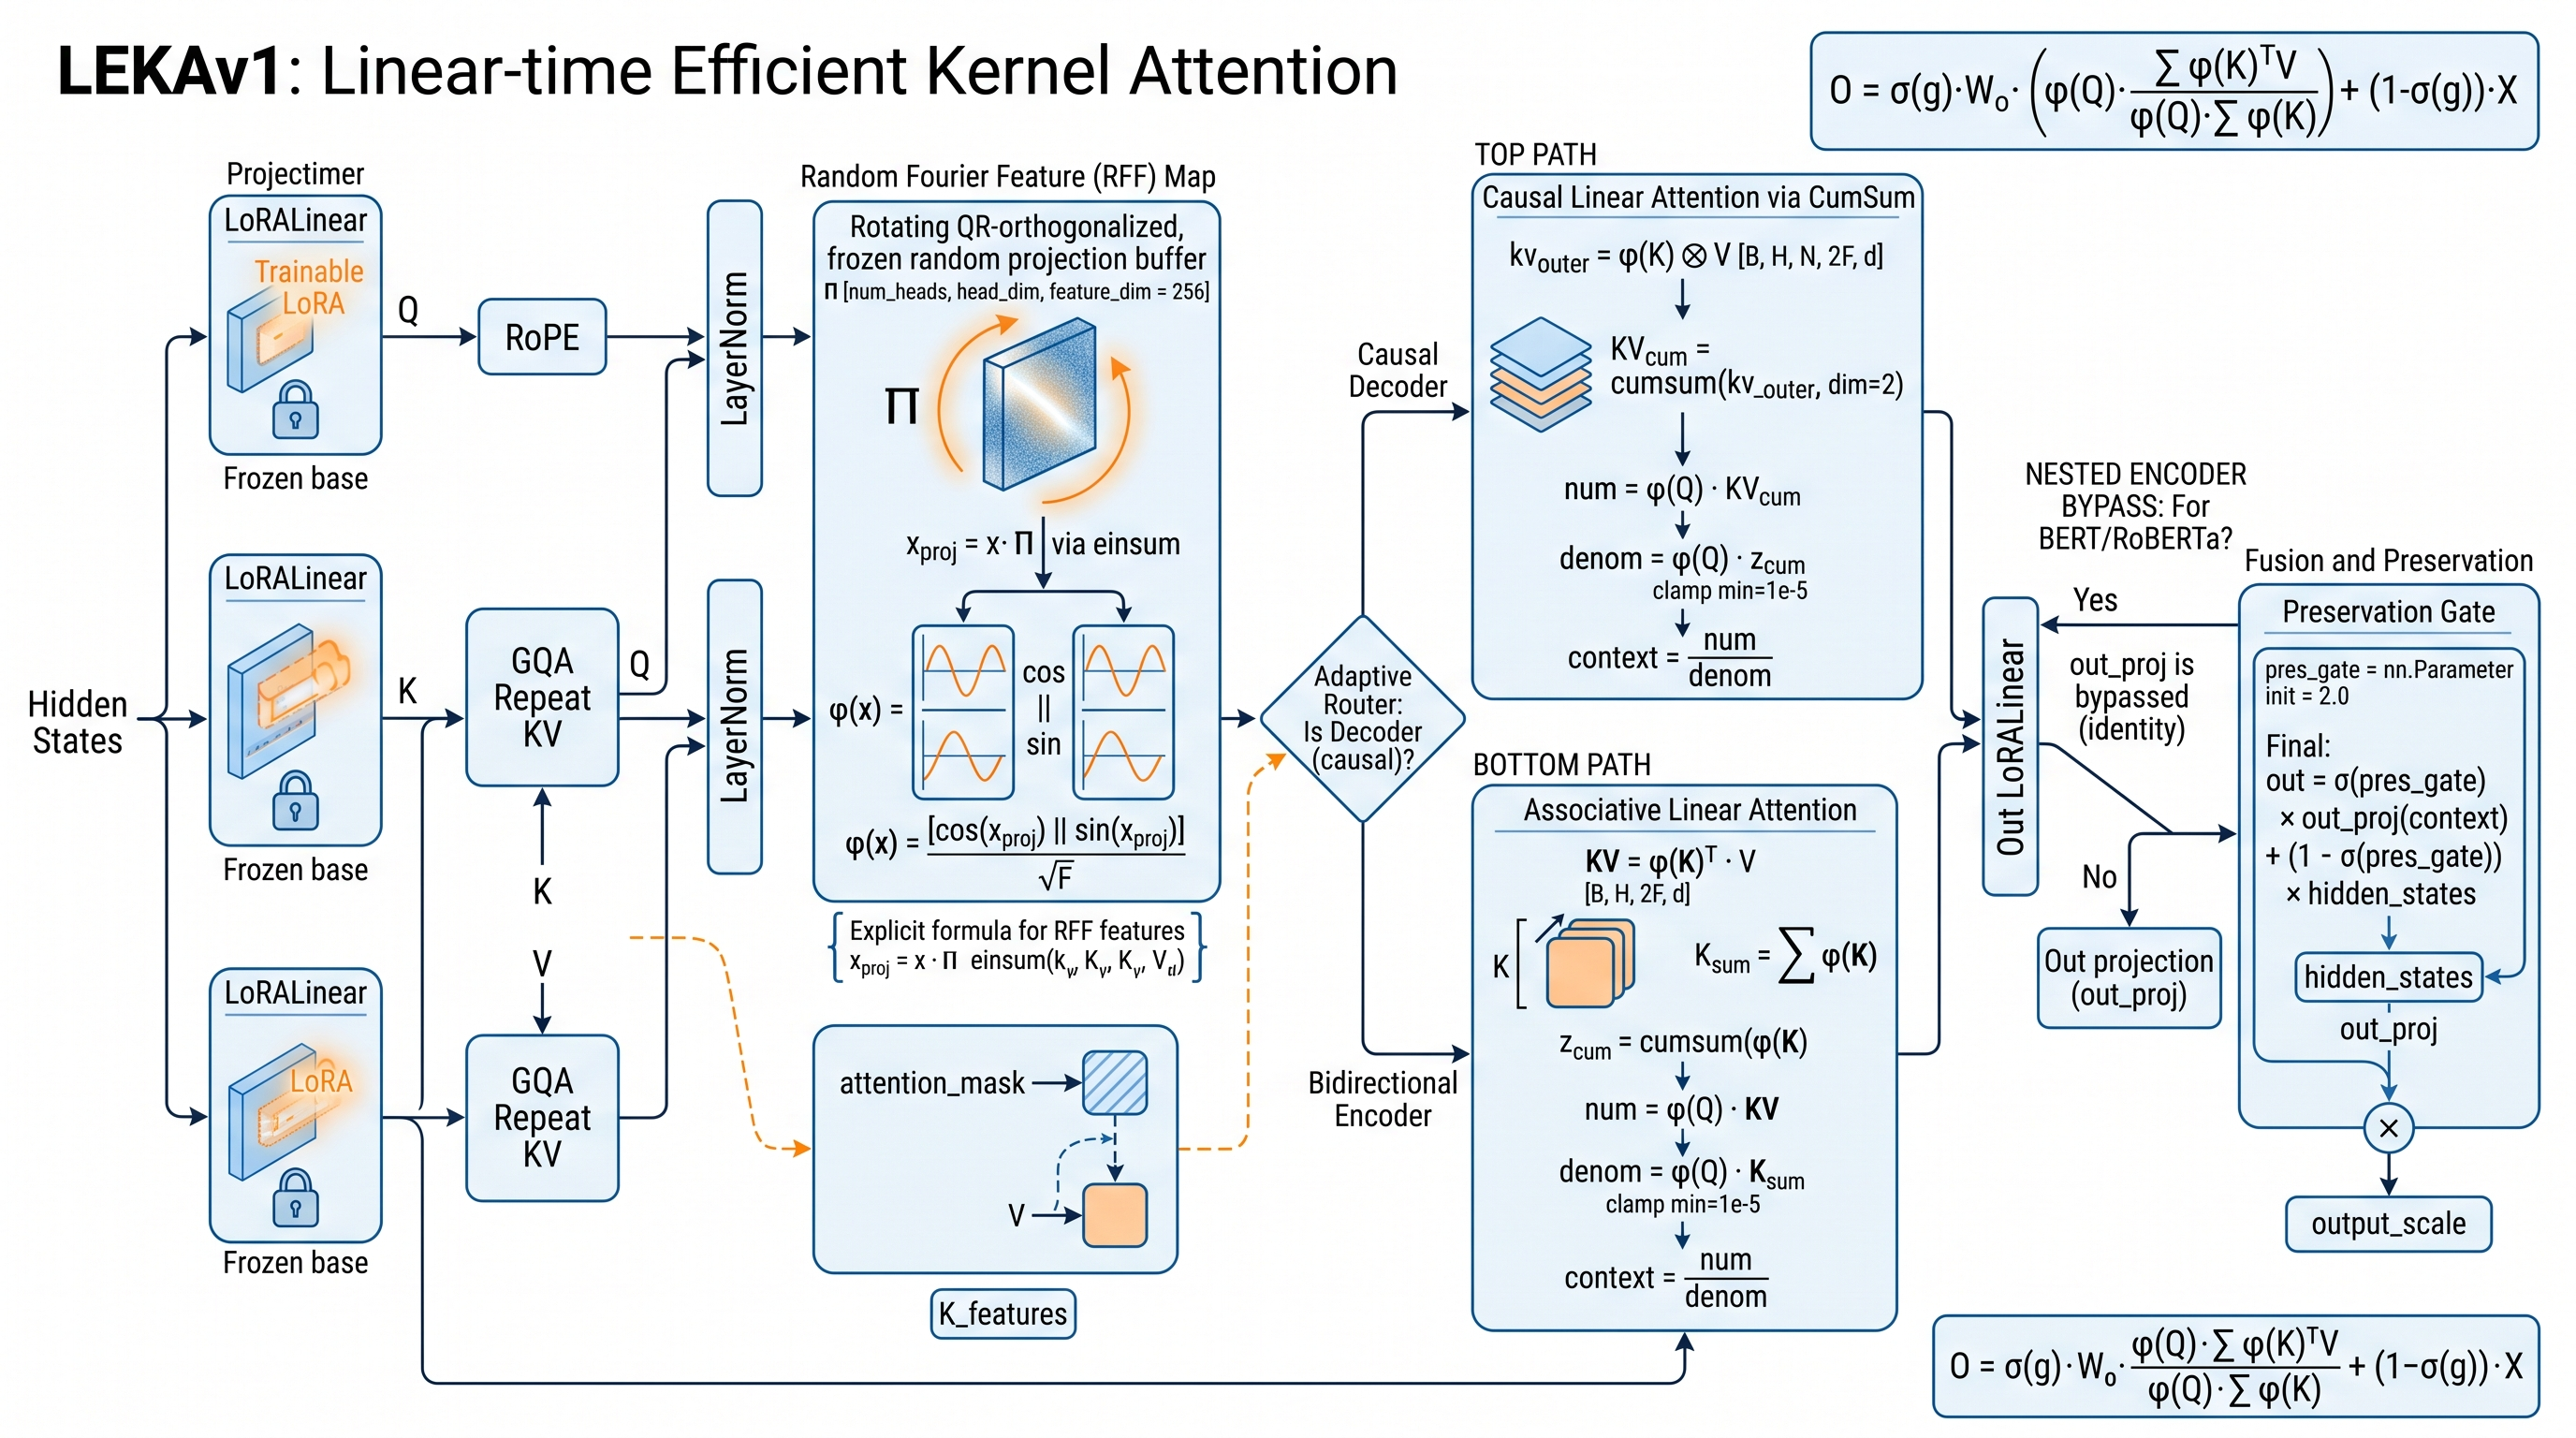
\includegraphics[width=\linewidth]{figures/architecture.jpeg}
\caption{High-level architectural diagram of leka\_v1.}
\label{fig:arch_leka-v1}
\end{figure}

